\subsection{Hardware test}
Now that the hardware has been chosen, it is necessary to test whether or not it lives up to its specifications.
The EV3 motors may have been used by many people before and could potentially have been damaged.
As such, it is important to test whether or not these motors will perform as advertised.

For each motor, both a precision test and a speed test have been performed.
The goal of the precision test is to determine how accurate the built-in rotation sensor is, while the speed test ascertains whether the rpm is accurate.
All motors were tested; the medium motor and both large motors.
The results will be presented starting with the medium servomotor, then the large left servomotor, and lastly the large right servomotor.

\subsubsection{Precision Test}
In order to test a motor's precision, the motor was instructed to turn a total of 360 degrees, after which the angle of the motor was noted with a dot on a measuring paper.
The setup can be seen in \autoref{fig:sssec:angle_test_setup}
This was done a total of 10 times for each motor, after which the spread of the angles were evaluated, to determine how much the angles had deviated.

\begin{figure}[H]
    \centering
    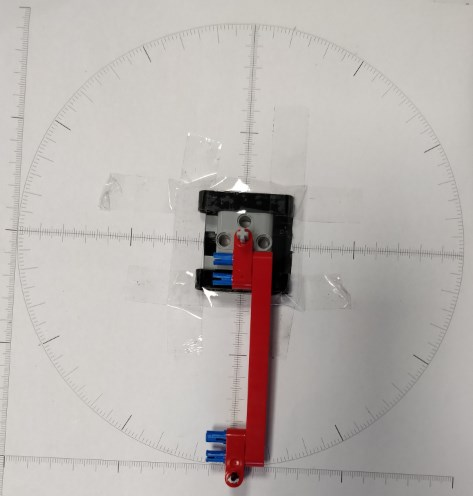
\includegraphics[scale = 0.5]{images/techAnalysis/MediumMotorAngleTest.jpg}
    \caption{The setup for testing the medium motor}\label{fig:sssec:angle_test_setup}
\end{figure}

The results of the tests showed that all motors stayed within its single degree accuracy, with the large left motor having the least amount of variance. The results for the medium motor can be seen in \autoref{fig:sssec:angle_test_result}

\begin{figure}[H]
    \centering
    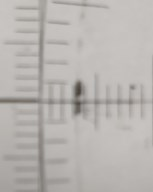
\includegraphics[scale = 0.8]{images/techAnalysis/MediumMotorAngleResult.jpg}
    \caption{Results from the precision test for the medium motor}\label{fig:sssec:angle_test_result}
\end{figure}

\subsubsection{Speed Test}
The speed test was conducted by instructing the motor to run at max speed for a total of six seconds.
This was recorded in slow-motion, and the number of rotations during this slow-motion video was manually counted.
The number of rotations counted during the six seconds can then be scaled up to one minute. 
A small lego brick was used to indicate the motor's starting position.
The physical setup for this test was the same as for the precision test.
This test was done five times for each motor.
The number of rotations was rounded to the nearest quarter-turn.

The results for the medium motor after running the speed test five times were:
24.75, 24.5, 26.25, 26.25, 26.0, this gives an average of 25.55 or 255 rpm.

The results for the large left motor after running the speed test five times were:
15.0, 15.75, 15.5, 15.0, 14.75, this gives an average of 15.2 or 152 rpm.

The results for the large right motor after running the speed test five times were:
15.5, 15.5, 14.5, 15.25, 16.0, this gives an average of 15.35 or 153 rpm.
\todo{reformat the visual presentation of the test-results}

Considering slight inaccuracies when scaling the results, the motors performed well within the specifications found in \autoref{ssec:motors}.
However it must be noted that during the test extra load was added, which could have had a impact on the result.
